%% $Id: prototype.tex,v 1.2 2000/05/09 16:56:03 matt Exp $

\chapter{Prototype}

\section{Indexer}
A prototype of the indexer was developed.  This was primarily to test out various indexing methods and have a chance to do some research into the area.  This research is shown in more detail later in Chapter \ref{techbasis}.

A lot of research has been done previously into the area of Information Retrieval, and several books \cite{wmb:mg, BasRib} and papers have been quite a useful base.

The prototype indexer was written in C and created compressed inverted indexes based on the \emph{Local Bernoulli Model} introduced by Witten et Al \cite{wmb:mg}.  These schemes use the fact that a list of document numbers are an increasing stream of integers with small intervals.  As such they can be represented in a much more compact form by storing the list of document numbers in which a particular word occurs as just a list of intervals.

This resulted in an average of just over 4 bits per index entry, compared to 32 or 64 bits if just storing the entry as an \texttt{int} or \texttt{long}.

The speed of the indexer was very impressive as well, resulting in around 3GB of text indexed per hour --  with 2-3 term ranked queries being answered in under a second.


\section{Front End}

\begin{figure}[!ht]
  \begin{center}
    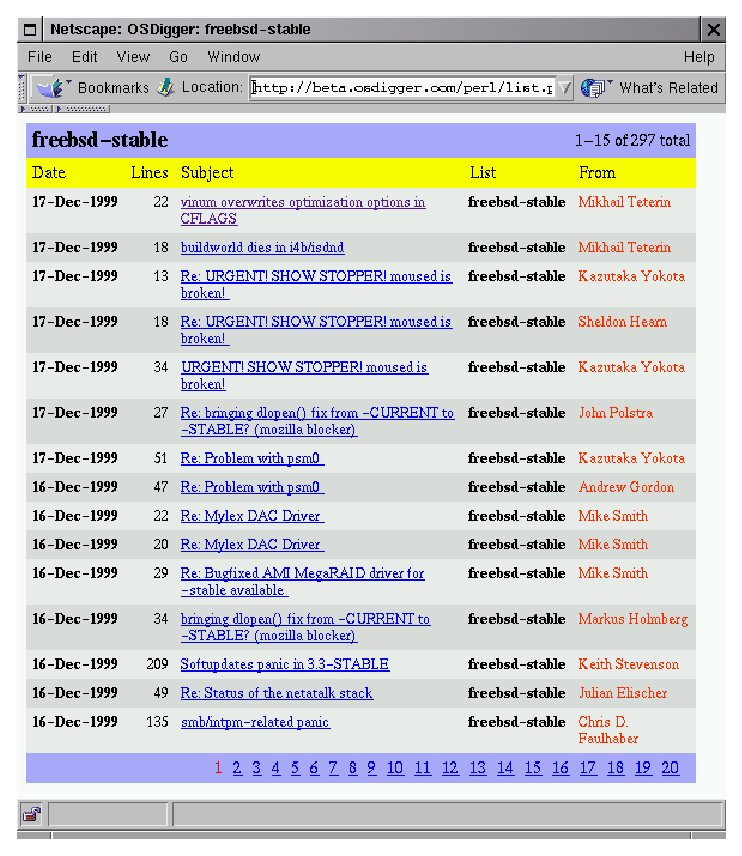
\epsfig{file=screen1.eps}
    \caption{Prototype Screenshot}
    \label{fig:screen1}
  \end{center}
\end{figure}

A simple web page was created using Perl and HTML to interact with the database.  A simple parser was written in Perl that would take a message in on standard input and insert it into the database.  The web page shows messages in a particular list sorted in reverse chronological order.  A screenshot of this interface can be seen in Figure \ref{fig:screen1}.

\pagebreak
\enlargethispage*{0.5cm}
\section{Conclusion}
From coding and using the prototype a number of points were discovered:

\begin{itemize}
\item The indexing algorithms discussed by Witten et Al will be fast enough for our needs.
\item Parsing messages is actually quite difficult, as there are so many standards out there and many mailers do not follow them all correctly.
\item Due to its great support for text manipulation, Perl seems like a good language to write both the parser and web scripts in.
\item The server supplied by Etherworks should have enough memory and CPU power to efficiently construct the indexes.
\end{itemize}

% LocalWords:  Witten int GB ht eps Screenshot Perl HTML
% LocalWords:  screenshot
